\documentclass[a0paper,portrait]{baposter}
\usepackage{myPreamble}
\usepackage{import}
\usepackage[backend=bibtex, sorting=none]{biblatex}
\addbibresource{mybib.bib}
\usepackage{lipsum}

\newtheorem{theorem*}{Theorem}
\definecolor{lightblue}{rgb}{0.1,0.46,0.72}
\definecolor{blue}{rgb}{0.1,0.46,1}

\begin{document}

\begin{poster}
{
columns=2,
headerborder=closed, % Adds a border around the header of content boxes
bgColorOne=white, % Background color for the gradient on the left side of the poster
bgColorTwo=white, % Background color for the gradient on the right side of the poster
boxColorOne=white, % Background color of the content boxes
headerColorOne=lightblue, % Background color for the header in the content boxes (left side)
headerColorTwo=lightblue, % Background color for the header in the content boxes (right side)
borderColor=lightblue, % Border color
headerFontColor=white, % Text color for the header text in the content boxes
textborder=roundedleft, % Format of the border around content boxes, can be: none, bars, coils, triangles, rectangle, rounded, roundedsmall, roundedright or faded
%eyecatcher=1, % Set to false for ignoring the left logo in the title and move the title left
headershape=roundedright, % Specify the rounded corner in the content box headers, can be: rectangle, small-rounded, roundedright, roundedleft or rounded
}
{}%left logo
{Modelling the Spread of COVID-19 Cases}
{\medskip\textsc{Anthony Gibbons}}
{
\includegraphics[width=6cm]{trinity-stacked.jpg}}

\headerbox{Introduction}{name=intro,column=0,row=0}{
The Coronavirus disease (COVID-19) was first characterized by the World Health Organisation as a pandemic on 11th March 2020. The outbreak has affected almost every aspect of human life throughout 2020, and is expected to continue for much of 2021. 

Situation in Ireland up to early 2021:

\begin{center}
\minipage{0.48\textwidth}
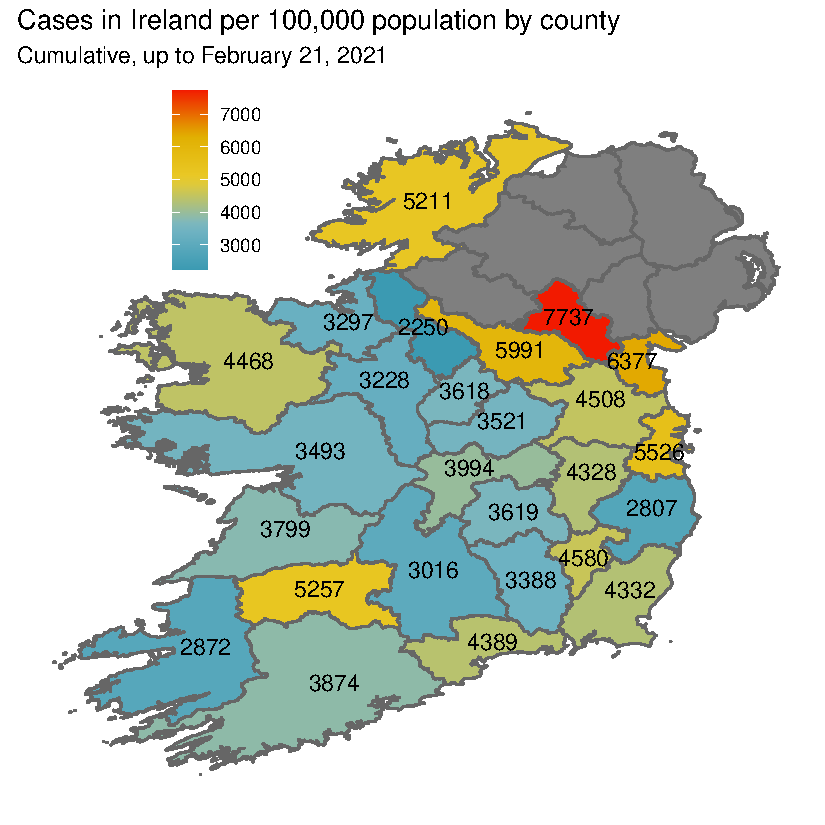
\includegraphics[width=0.9\textwidth]{county-rep.pdf}
\endminipage\hfill
\minipage{0.48\textwidth}
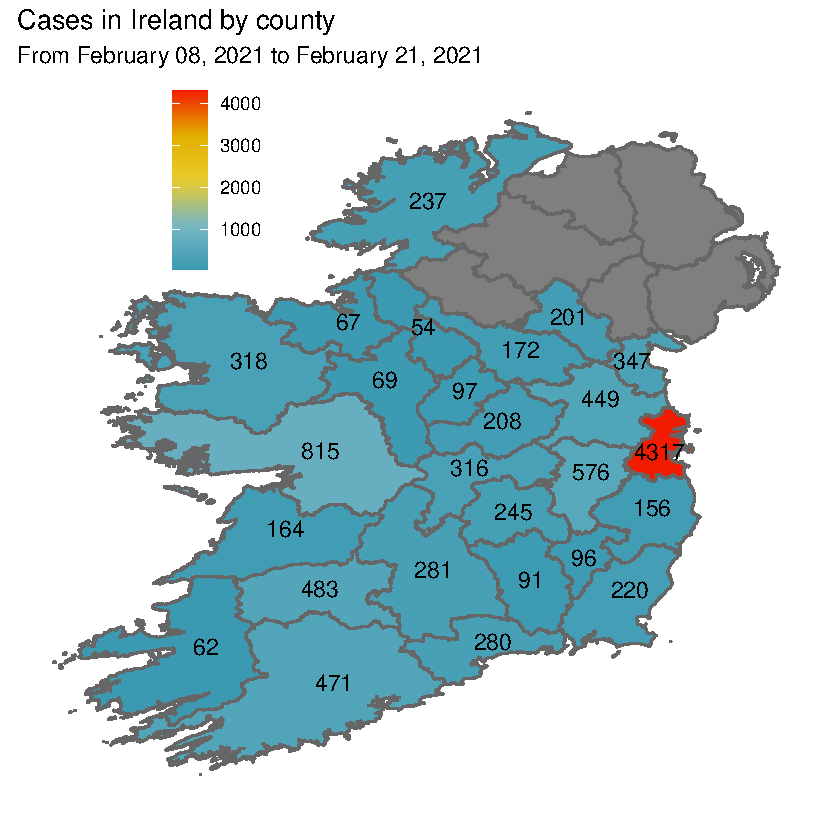
\includegraphics[width=0.9\textwidth]{county-fourteendaycases.pdf}
\endminipage
\end{center}
}

\headerbox{Mathematical Models}{name=box1,column=0,below=intro}{
Based on methods derived in \cite{grigor20}.

\textbf{Model Assumptions}
\begin{itemize}
    \item[(I)] Any infected person becomes ill (symptomatic) and infectious on the $q$-th day after infection.
    \item[(A)] During each day, each ill person unconfined infects on average $a$ other persons.
    \item[(B)] During each day, a proportion $b\in (0,1)$ of ill people loose gets isolated and withdrawn from a further spread of the epidemic.
\end{itemize}

We derive the recurrence relation 

\begin{equation} \label{eq:xnrecurr}
    x_{n+1} = (1 - b) x_n + ax_{n-q}, \quad x_n = x^*_n \ \text{for} \ n = 0, 1, \dots , q.
\end{equation}

The recurrence equation has limiting behavior:
 \begin{equation}\label{eq:crn}
        x_n \sim Cr^n \text{ as } n\to\infty.
    \end{equation}

For the periodic model, we allow for some oscillation of the parameters $a$ and $b$:

\begin{equation} \label{eq:anper}
a_n := a\rbr{1+c_1\rbr{\sin\rbr{\frac{2\pi}{p_1}\rbr{n-n_1}}}}
\end{equation}

\begin{equation} \label{eq:bnper}
b_n := b\rbr{1+c_2\rbr{\sin\rbr{\frac{2\pi}{p_2}\rbr{n-n_2}}}}
\end{equation}

}

\headerbox{Limiting Curve}{name=box2,column=0,below=box1}{

\begin{center}
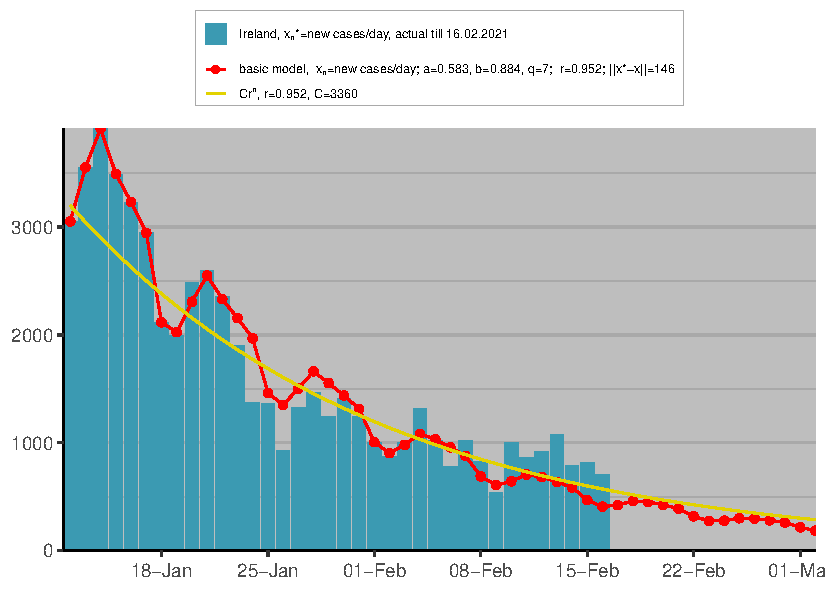
\includegraphics[width=0.9\textwidth]{Ireland-Crn.pdf}
\end{center}
}


\headerbox{Base and Periodic Models}{name=box3,column=1}{%,aligned=intro}{
\begin{center}
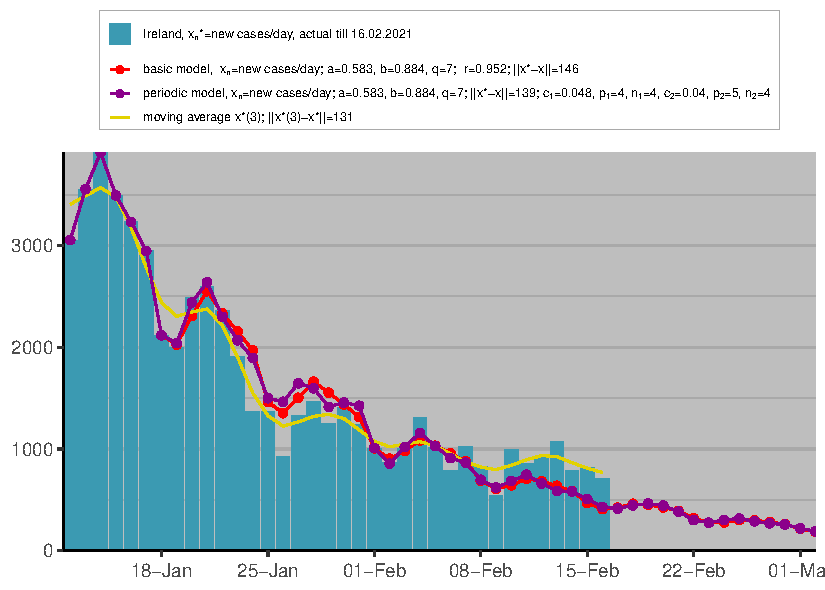
\includegraphics[width=0.8\textwidth]{Ireland-periodic.pdf}
\end{center}
}

\headerbox{Statistical Models}{name=box4,column=1,below=box3}{
Based on time series forecasting methods discussed in \cite{Hyndman-et-al-2018}.

Statistical models give us some more information to work with in the form of confidence intervals for the forecast period.
}

\headerbox{Seasonal ARIMA Model}{name=box5,column=1,below=box4}{
\begin{center}
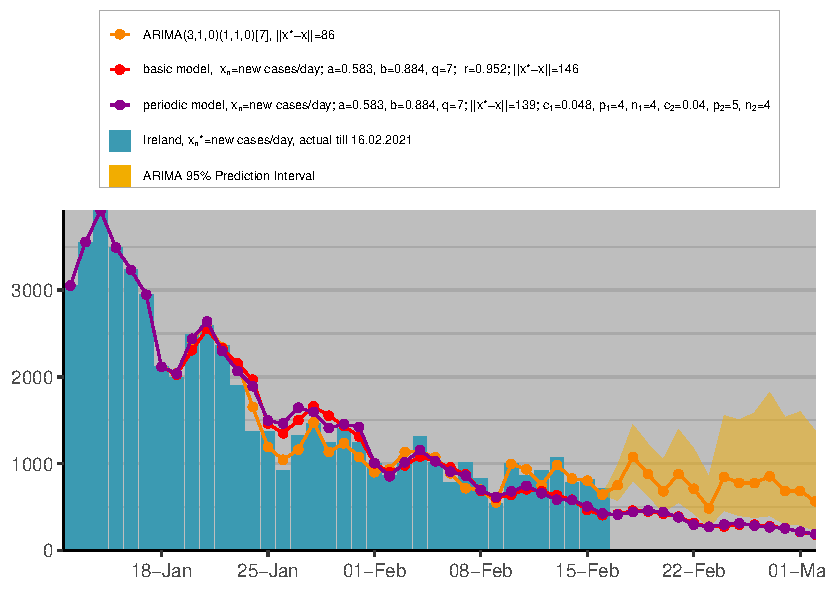
\includegraphics[width=0.8\textwidth]{Ireland-arima.pdf}
\end{center}
}

\headerbox{Seasonal Holt-WInters' Model}{name=box6,column=1,below=box5}{
\begin{center}
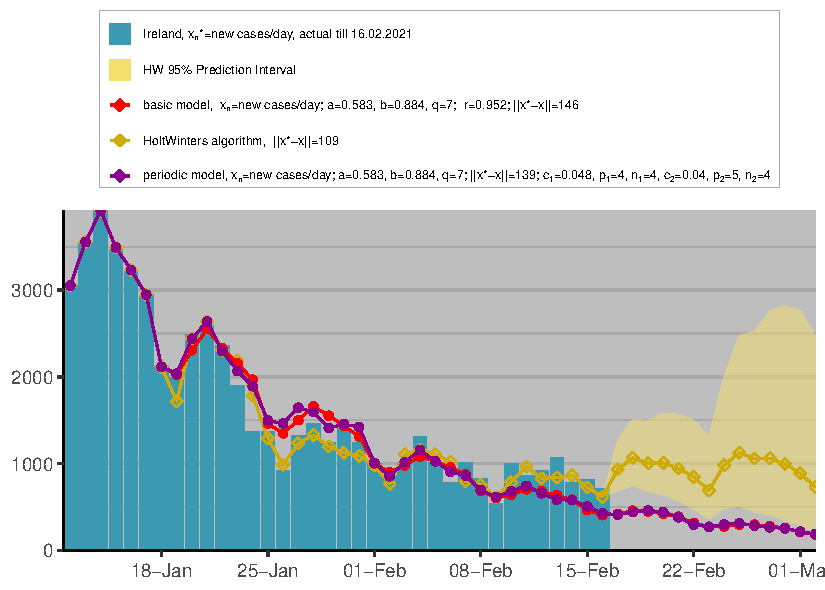
\includegraphics[width=0.8\textwidth]{Ireland-hw.pdf}
\end{center}
}

\headerbox{References}{name=ref,column=1,below=box6}{
\printbibliography[heading=none]
}

\end{poster}
\end{document}